\subsubsection{Если транзистор имеет большой разброс коэффициентов усиления по току B, то на каких параметрах это скажется?}

Рассмотрим 3 каскада и их коэффициенты усиления:
1) Каскад ОЭ (вставляем схему и рассчитываем $R_{in},K_{U}$):
$$
K_{U}=\frac{B*R_{k}//R_{n}}{r_{e}*(B+1)+r_{b}}
$$
Если $r_{b}$ мало, то:
$$
K_{U}=\frac{B*R_{k}//R_{n}}{r_{e}*(B+1)}\approx \frac{R_{k}//R_{n}}{r_{e}}
$$
то есть $K_{U}$ не зависит от В, где $B=\frac{I_{k}}{I_{b}}$ -> показывает во сколько раз ток коллектора больше тока базы.
Пусть $R_{n}\to\infty$ ($R_{r}=0$):
$$
K_{U}=\frac{R_{k}}{r_{e}}
$$
$$
r_{e}=\frac{\varphi_{T}}{I_{E.rab.tochk}}
$$
Теперь преобразуем $K_{U}$ с учётом $\alpha=\frac{B}{B+1}$
$$
K_{U}=\frac{\alpha*R_{k}*I_{E.rab.tochk}}{\varphi_{T}}=\frac{R_{k}*I_{k}}{\varphi_{T}}=\frac{E_{k}}{2*\varphi_{T}}
$$
Это возможно только, если потенциал в точке 1 будет равен $\frac{E_{k}}{2}$
\begin{center}
\begin{figure}[h!]
\center{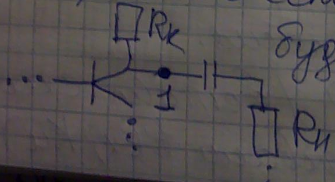
\includegraphics[scale=0.7]{p3_21.png}}
\end{figure}
\end{center}
$$
K_{IOE}=\frac{R_{b}*B*R_{kn}}{R_{b}+r_{b}+r_{e}*(B+1)}\approx \frac{R_{b}*R_{kn}}{\frac{R_{b}+r_{b}}{B}+r_{e}}\approx \frac{R_{b}*R_{kn}}{r_{e}}
$$

2)Каскад ОБ (аналогично вставляем схему и рассчитываем $R_{in},K_{U}$):
$$
K_{U}=\frac{B*R_{kn}}{R_{in.tr.OE}}
$$
если $r_{b}$ мало, то 
$$
K_{U}=\frac{B*R_{kn}}{r_{e}*(B+1)}\approx \frac{R_{kn}}{r_{e}}
$$
Не зависит от В.
$$
K_{IOВ}=\frac{R_{E}*\alpha*R_{kn}}{R_{E}+\frac{R_{in.tr.}}{(B+1)}}
$$
$$
\frac{R_{вх.тр.}}{(B+1)}=\frac{r_{b}}{(B+1)}+r_{e}\approx r_{e}\to 0
$$
следовательно:
$$
K_{IOВ}=\frac{R_{E}*\alpha*R_{kn}}{R_{E}+1}
$$

3) Каскад ОК (всё аналогично):
$$
K_{U}=\frac{R_{En}*(B+1)}{r_{b}+r_{e}*(B+1)+R_{En}*(B+1)}\approx \frac{R_{En}}{r_{e}+R_{En}}
$$
следовательно не зависит от В.
$$
K_{IOK}=\frac{R_{b}*(B+1)*R_{e}}{[R_{b}+R_{in.tr.}+R_{En}*(B+1)]*(R_{e}+R_{n})}=
$$
$$
=\frac{R_{b}*(B+1)*R_{e}}{(B+1)[\frac{R_{b}+r_{b}}{B+1}+r_{e}+R_{En}]*(R_{e}+R_{n})}=\frac{R_{b}*R_{e}}{(r_{E}+R_{En})(R_{E}+R_{n})}
$$
